\documentclass{standalone}
\usepackage{tikz}
\usepackage{float}
\usepackage{amsmath}
\usepackage{lmodern}
\usepackage{amssymb}
\usetikzlibrary{calc}
\usetikzlibrary{hobby}
\usetikzlibrary{decorations.markings}
\usetikzlibrary{patterns, patterns.meta}
\usetikzlibrary{shapes}
\usepackage{pgfplots}

\pgfplotsset{compat=1.18}
\begin{document}

\centering

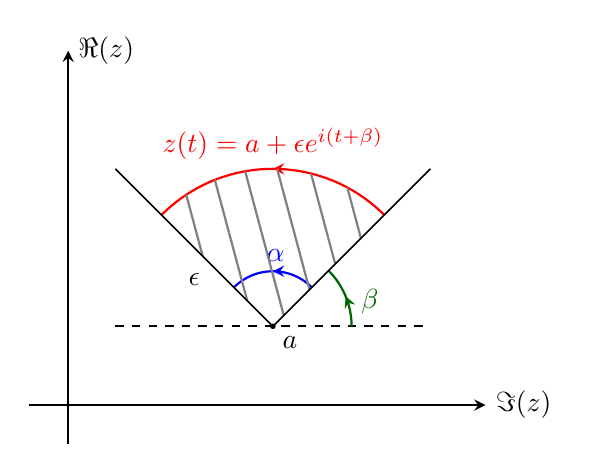
\begin{tikzpicture}
    \tikzset{
    % style to apply some styles to each segment of a path
    on each segment/.style={
      decorate,
      decoration={
        show path construction,
        moveto code={},
        lineto code={
          \path [#1]
          (\tikzinputsegmentfirst) -- (\tikzinputsegmentlast);
        },
        curveto code={
          \path [#1] (\tikzinputsegmentfirst)
          .. controls
          (\tikzinputsegmentsupporta) and (\tikzinputsegmentsupportb)
          ..
          (\tikzinputsegmentlast);
        },
        closepath code={
          \path [#1]
          (\tikzinputsegmentfirst) -- (\tikzinputsegmentlast);
        },
      },
    },
    % style to add an arrow in the middle of a path
    mid arrow/.style={postaction={decorate,decoration={
          markings,
          mark=at position .5 with {\arrow[#1]{stealth}}
        }}},
  }
  \tikzset{arrowstyle/.style={->, >=stealth}}
    % draw axes
    \coordinate (O) at (0,0);
    \draw[arrowstyle, thick] (0,-0.5) -- (0,4.5) node[anchor=west] {$\Re (z)$};
    \draw[arrowstyle, thick] (-0.5,0) -- (5.3,0) node[anchor=west] {$\Im (z)$};

    \begin{scope}[xshift=-0.4cm, yshift=-1.0cm]
      % draw point a
      \coordinate (p1) at (3,2);
      \fill (p1) circle (1pt);
      \draw (p1) node[below right] {$a$};
      % draw reference horizontal line
      \draw[dashed, line width = 0.5pt,thick] ($(p1) + (-2, 0)$) -- ($(p1) + (2, 0)$);

      % draw arcs
      \path [draw=red,thick,postaction={on each segment={mid arrow=red}}]
      (p1) ++(45:2) arc[start angle=45, end angle=135, radius=2];
      \path [draw=black!60!green,thick,postaction={on each segment={mid arrow=black!60!green}}]
      ($(p1)+(1,0)$) arc[start angle=0, end angle=45, radius=1];
      \path [draw=blue,thick,postaction={on each segment={mid arrow=blue}}]
      (p1) ++(45:0.7) arc[start angle=45, end angle=135, radius=0.7];

      % labels arcs
      \draw[color=black!60!green] ($(p1) + (1, 0.6)$) node[below right] {$\beta$};
      \draw[color=red] ($(p1) + (0,2)$) node[above] {$z(t) = a + \epsilon e^{i(t+\beta)}$};
      \node at ($(p1) + (1pt,0.9)$) [draw=white, circle, inner sep=0, fill=white] {\textcolor{blue}{$\alpha$}};


      % draw hatched pattern
      \fill[thick,pattern ={Lines[angle=105, distance=0.4cm]},pattern color=gray] (p1) -- ++(45:2) arc[start angle=45, end angle=135, radius=2] -- cycle;

      \draw[semithick] (p1) -- ($(p1) + (2, 2)$);
      \draw[semithick] (p1) -- ($(p1) + (-2, 2)$) node[pos=0.4, below left] {$\epsilon$};
    \end{scope}

\end{tikzpicture}
\end{document}